\label{sec:rq3}
\textbf{Motivation.} RQ1 and RQ2 show \emph{that} the agents' issues differ; they do not show what the issues are about. Studies of agent pull requests suggest that developers hand agents particular kinds of work, such as refactoring, documentation and testing~\cite{watanabe2025agentic}. If the same holds for issues, topics can explain part of the differences in closure and speed, and they tell maintainers what work to expect from each agent.

\textbf{Approach.} \emph{Corpus.} The topic models cover the \NEnglishTested{} English issues of the eleven tested agents. Each document is the issue title and body after removing code blocks, links, HTML, user mentions, template text (lines repeated verbatim in at least ten issues) and every agent name and signature, so that a topic cannot simply restate the agent label. Tokens were lemmatised and frequent word pairs joined, and only terms were kept that occur in at least ten documents and at most half of them. Documents with fewer than ten tokens were dropped, which leaves \NDocsRQThree{} documents (median \MedTokens{} tokens) and \NVocab{} terms.

\emph{Single LDA runs.} LDA~\cite{blei2003lda} is the most widely used topic model in software-engineering research~\cite{chen2016survey,silva2021topic}, so the analysis started there. It was fitted for \(k = 5\) to 20 topics with three random seeds each, and C\textsubscript{v} coherence~\cite{roder2015coherence} was measured. Coherence hardly changes with \(k\) (\CvMin\ to \CvMax), so it cannot single out one model. A bigger problem is that the topics are not reproducible: when a model is refitted with another seed, at most \SelRepro\% of the topics of the best model (\(k = \SelK\), C\textsubscript{v} = \SelCv) and at most \SingleReproMax\% for any \(k\) reappear, where a topic counts as reappearing if at least seven of its ten top words recur in the matched topic~\cite{greene2014stability}. A topic list from a single run would therefore partly reflect the random seed, a risk that Agrawal et al.\ warned about for software-engineering data~\cite{agrawal2018wrong}.

\emph{Ensemble LDA at two levels.} The study therefore uses Ensemble LDA~\cite{brigl2019ensemble}, which fits many models (here 16) and keeps only the topics that recur across them, with two independent ensembles fitted with different seeds. Under the rule fixed in advance, which chooses the clustering threshold that maximises the number of topics reproduced by both ensembles, \NTopicsH{} topics remain; they form the \emph{headline} level. Two topics are coarse, so the paper also reports a \emph{fine} view: the threshold at which both ensembles find the most topics (\NTopicsF). The researcher defined this second rule after seeing the headline result, so every fine topic is graded by how many of its ten top words recur in the matching topic of the other ensemble: \emph{reproduced} (seven or more), \emph{partly reproduced} (five or six) or \emph{not reproduced} (fewer than five).

\emph{Labels and their validation.} Each topic was labelled after reading its top words and its most representative issues, and the researcher then checked the labels of the fine topics on five random issues per topic, judging for each whether the label describes it. Before the check, the rule was set that a label fails if two or more of its five issues do not fit. A fine topic is interpreted only if it is reproduced \emph{and} its label passes this check.

\emph{Triangulation with BERTopic.} Recent studies of agent pull requests and of issue trackers use BERTopic~\cite{opu2025performance,das2024chatgpt,grootendorst2022bertopic}, which clusters documents by meaning rather than by word co-occurrence. To test whether the conclusions depend on the method, the same documents were also clustered with BERTopic: sentence embeddings~\cite{reimers2019sbert} of the whole issue (long issues are embedded in 150-word chunks that are then averaged), dimensionality reduction with UMAP~\cite{mcinnes2018umap}, and \(k\)-means with as many clusters as the fine view has topics, repeated with three seeds.

\begin{table*}[t]
\caption{RQ3 topics at the headline level (H) and in the fine view (T). Shared = top-10 words that recur in the matching topic of the second, independent ensemble; Prev.\ = share of all topic weight (\%)}\label{tab:rq3}
\centering\footnotesize\setlength{\tabcolsep}{3pt}
\begin{tabular}{@{}l l r r l@{}}
\toprule
& Label & Shared & Prev. & Top words\\
\midrule
\inputtab{generated/tab_rq3_topics.tex}
\bottomrule
\end{tabular}
\end{table*}

\textbf{Results.} \emph{Topics.} At the headline level, the issues split into code maintenance and quality work (H1) and AI and LLM tooling and research (H2), both reproduced across ensembles (Table~\ref{tab:rq3}). In the fine view, two topics meet both conditions for interpretation: testing, review and quality follow-ups (T1; label fits \ValFitOneK{} of \ValFitOneN{} sampled issues) and code-level fixes and refactoring (T4; \ValFitFourK{} of \ValFitFourN). The other three fine topics are not interpreted. T2, whose words suggest implementation plans and integration phases, does not recur in the second ensemble. T3 and T5 recur only partly, and their labels failed the check (\ValFitThreeK{} and \ValFitFiveK{} of 5 issues fit): the sampled issues ranged from a thermostat bug to a payment-channel problem, so these two word lists do not describe a coherent kind of work.

\emph{Topics depend on the agent.} The topics of an agent's issues depend on the agent (Fig.~\ref{fig:rq3heat}). The association is \EffTHMain{} at the headline level (V = \VTHMain) and at the border between medium and large in the fine view (V = \VTFMain, where the threshold for a large effect is 0.25). It holds for human-authored issues only (S2, V = \VTFSTwo), on the precision subset (S3, V = \VTFSThree) and when the documents of the non-reproduced topic are left out (V = \VTFStable). It is much weaker, though still significant, when the ensemble is refitted on a corpus that also contains very short issues of five to nine tokens: the topics then change, and V drops to \VTFFive{} in the fine view and \VTHFive{} at the headline level.

\begin{figure*}[t]
\centering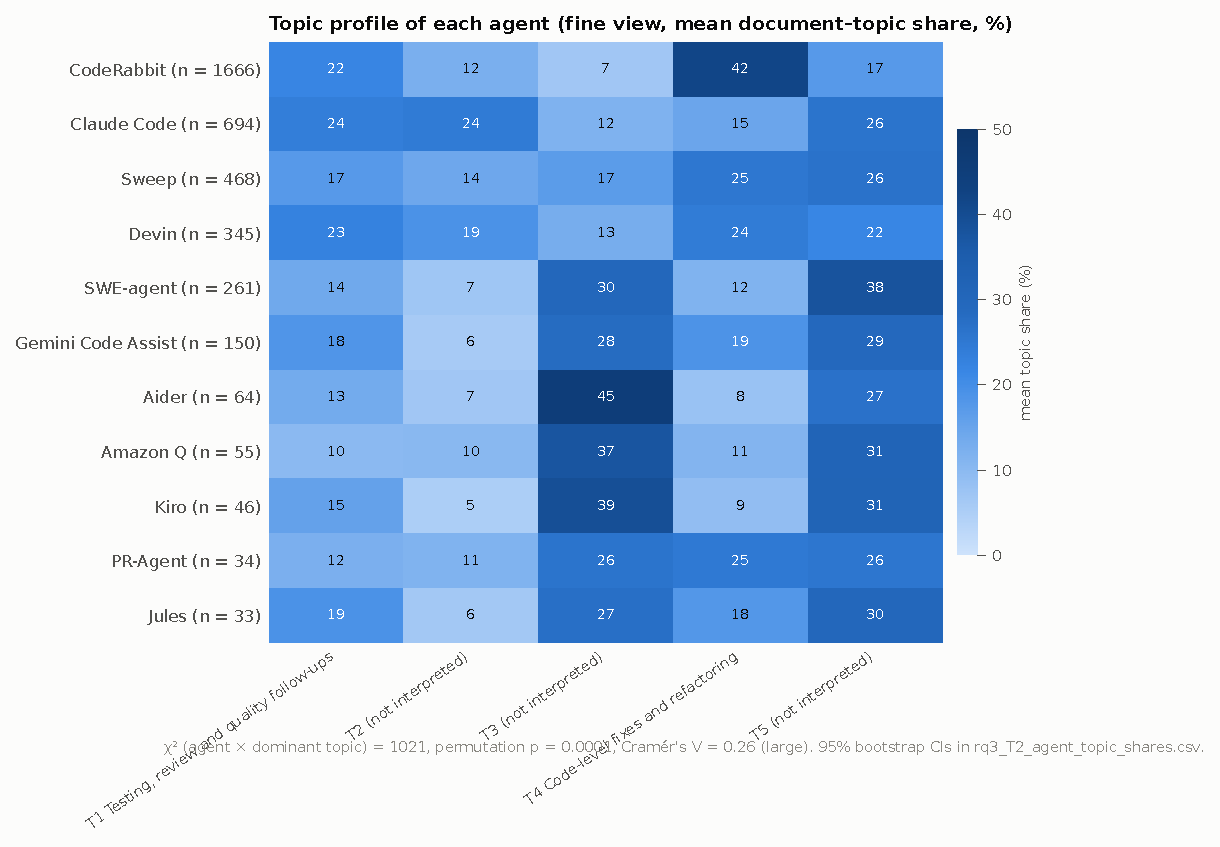
\includegraphics[width=0.62\textwidth]{rq3_R2_agent_topic_heatmap.pdf}
\caption{Topic profile of each agent in the fine view: mean share of each topic in the agent's issues (\%).}\label{fig:rq3heat}
\end{figure*}

\emph{Which agents drive it.} Adjusted residuals beyond \(|z| = \ZCritFine\) (Bonferroni) count as significant, and they are read only for the interpreted topics. CodeRabbit shows the clearest pattern. Its issues are strongly over-represented in code-level fixes (\(z = \ResCodeRabbitCode\), and \(z = \ResSThreeCodeRabbitCode\) on the precision subset), which make up \ShareCodeCodeRabbit\% of the topic weight of its issues (95\% bootstrap CI \ShareCodeCodeRabbitCI), and it wrote \CodeTopicShareCodeRabbit\% of the issues dominated by this topic although it accounts for \DocShareCodeRabbit\% of the documents. The pattern comes from the issues CodeRabbit writes itself: \CodeRabbitOwnPRRef\% of them refer to a pull request or a review, and code-level fixes make up \CodeShareOwnCodeRabbit\% of their topic weight, against \CodeShareOtherCodeRabbit\% for CodeRabbit's other issues. These are the issues that RQ1 showed are often left open.

\emph{Triangulation.} BERTopic is far more stable than LDA: all of its topics recur across seeds (adjusted Rand index between seeds \BTAriMin\ to \BTAriMax). It confirms the main conclusion: topics depend on the agent, with a \BTEff{} effect (V = \BTV, and \BTVMin\ to \BTVMax\ across seeds). On BERTopic's own topics, CodeRabbit is again over-represented in code-level work (\(z = \BTResCodeRabbitCode\)). The two methods divide the corpus differently, however. Matched topics share few top words (mean Jaccard \TriWordJ), and agreement at the level of single issues is low (adjusted Rand index \TriARI; \TriSame\% of issues fall in the matched topic).

\emph{Topics and time-to-close.} Time-to-close differs only slightly between the fine topics (\(\varepsilon^2 = \TopicKWeps\), \TopicKWeff; log-rank \(p = \TopicLRp\)). Code-level fixes have the longest Kaplan--Meier median (\KMDaysCode{} days) and build and workflow issues the shortest (\KMDaysWorkflow{} days). Because two-thirds of the code-level issues come from CodeRabbit, this difference cannot be separated from the agent.

\rqsummary{RQ3}{Agents raise different kinds of work. The association holds under two topic models, across seeds and on the S2 and S3 subsets, but it weakens when very short issues are included. The clearest case is CodeRabbit: its own issues are follow-ups from pull-request reviews, code-level fixes, a topic that is reproduced and whose label passed manual validation, are their largest topic, and CodeRabbit's issues lean towards code-level work under both topic models. Only two of the five fine topics, however, are both reproducible and correctly labelled, and LDA and BERTopic divide the same issues differently. Topic-modelling studies of agent artefacts should therefore check topic stability, validate topic labels by hand, and confirm their conclusions with a second method before interpreting individual topics.}
